
\chapter{Data Aggregation}
First step towards this project is to fetch our data from Twitter. The data is classified into two
groups, relevant and irrelevant. We will be spending most of our time with the relevant data.


\section{Data Classification}
To carry out our experiments, we will need to filter out irrelevant tweets. Irrelevant tweets are
tweets which we do not really care about. Some examples include:

\begin{itemize}
  \item \textit{Every day I'm levelling! And now I'm level 19 in \#CSRClassics for iPhone! Get it for FREE!}
  \item \textit{Yes, our apple juice and cider are both GMO-free.}
  \item \textit{I just had my first carmel apple}
\end{itemize}

Both tweets could be regarded as relevant but for our use case, they are not. This is because we are
only interested in tweets that contain personal opinions about Apple Incorporated. Examples of
relevant tweets include:
their thoughts
\begin{itemize}
  \item \textit{Once you get hooked to \#Mac, you will definitely go back to \#Windows! Lol!}
  \item \textit{If Tim Cook at Apple knows anything about him, it'd be to stay away from Icahn.}
\end{itemize}

Of course we can manually classify this data but when we have millions of tweets, this becomes
impracticable. This is where we employ some classification algorithms to assist us. This is a
three step process and we will discuss them in the next sub sections.

\subsection{Preparing train data}
Train data, also known as a training set is a set of data used to train a knowledge database, in
this case, a classifier. There are two main ways of getting a training set and they are
\begin{enumerate*}
  [label=\itshape\alph*\ushape{)}]
  \item creating a new set of data
  \item labelling a fraction of the actual data
\end{enumerate*}

For our purposes, we use the former because we are dealing with natural language and not numbers.
People write in different ways on Twitter and trying to create a new training set to encompass all
possibilities would be very time consuming.

I created an application to assist with labelling our train data. It can be found at
\url{http://bit.ly/data\_labeller} and a screen shot has been provided in Figure~\ref{fig:labeller}

\begin{figure}
  \begin{center}
    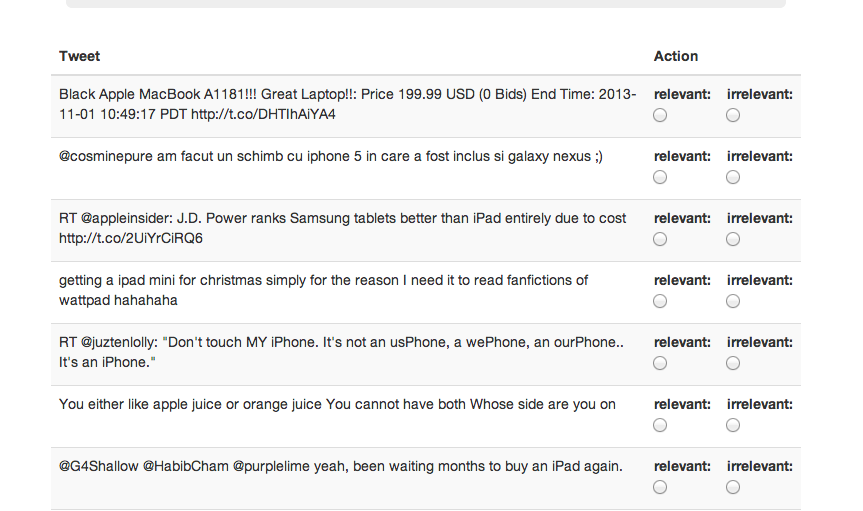
\includegraphics[scale=0.4]{figures/datalabeller}
  \end{center}
  \caption{The data labelling application}
\label{fig:labeller}
\end{figure}


\subsection{Choosing and training a classifier}
A Naive Bayes Classifier is a probabilistic classifier which is mainly based on the Bayes Theorem.
The classifier works on the assumption that the presence or absence of two features are
stochastically independent.

We will train a Naive Bayes Classifier and use it to classify the tweets into relevant and
irrelevant groups. \textbf{This work is currently in progress}

\subsection{Classifying tweets}
